\documentclass[[12pt,oneside,openany,a4paper, %... Layout
english, %... Global lang drivers{}
masters-t, goldenblock]{usthesis} 
\usepackage{graphicx}
% \usepackage[colorinlistoftodos,prependcaption,textsize=small,disable]{todonotes}
\usepackage[colorinlistoftodos,prependcaption,textsize=small]{todonotes}
\usepackage{pgfgantt}
\usepackage{float} %so that it can use the 'f' float option
\usepackage{pdflscape} %allow you to make landscape pages
\usepackage{amsmath}
\newcommand*\mean[1]{\bar{#1}} % to create an overbar for symbols
% \usepackage{cite}
\usepackage{soul}
\usepackage{amssymb}
\usepackage{bm}
\usepackage{standalone}
\usepackage{preview}
\usepackage{mathtools}
\usepackage{pdfpages}
% \usepackage[sort&compress]{natbib} %able to cite 2 reference at once
\usepackage{cite}
% \usepackage{gensymb} %for degree symbol
% \usepackage{hyperref} %to hyperlink the equations

\newganttlinktype{drur}{
\ganttsetstartanchor{on bottom=0.75}
\ganttsetendanchor{on left}
\draw [/pgfgantt/link]
% first segment (down)
(\xLeft, \yUpper) --
% second segment (right)
(\xLeft, \yUpper -
\ganttvalueof{link bulge} * \ganttvalueof{y unit chart}) --
% link label
node [pos=.5, /pgfgantt/link label anchor] {\ganttlinklabel}
% third segment (up)
($(\xLeft,
\yUpper -
\ganttvalueof{link bulge} * \ganttvalueof{y unit chart})!%
\ganttvalueof{link mid}!%
(\xRight,
\yUpper -
\ganttvalueof{link bulge} * \ganttvalueof{y unit chart})$) --
% last segment (right again)
($(\xLeft, \yLower)!%
\ganttvalueof{link mid}!%
(\xRight, \yLower)$) --
(\xRight, \yLower);
}

\newganttlinktype{rdldr*}{%
  \draw [/pgfgantt/link]
    (\xLeft, \yUpper) --
    (\xLeft + \ganttvalueof{link bulge 1} * \ganttvalueof{x unit},
      \yUpper) --
    ($(\xLeft + \ganttvalueof{link bulge 1} * \ganttvalueof{x unit},
      \yUpper)!%
      \ganttvalueof{link mid}!%
      (\xLeft + \ganttvalueof{link bulge 1} * \ganttvalueof{x unit},
      \yLower)$) --
    ($(\xRight - \ganttvalueof{link bulge 2} * \ganttvalueof{x unit},
      \yUpper)!%
      \ganttvalueof{link mid}!%
      (\xRight - \ganttvalueof{link bulge 2} * \ganttvalueof{x unit},
      \yLower)$) --
    (\xRight - \ganttvalueof{link bulge 2} * \ganttvalueof{x unit},
      \yLower) --
    (\xRight, \yLower);%
}
\ganttset{
  link bulge 1/.link=/pgfgantt/link bulge,
  link bulge 2/.link=/pgfgantt/link bulge}

\begin{document}

\includepdf{Cover.pdf}
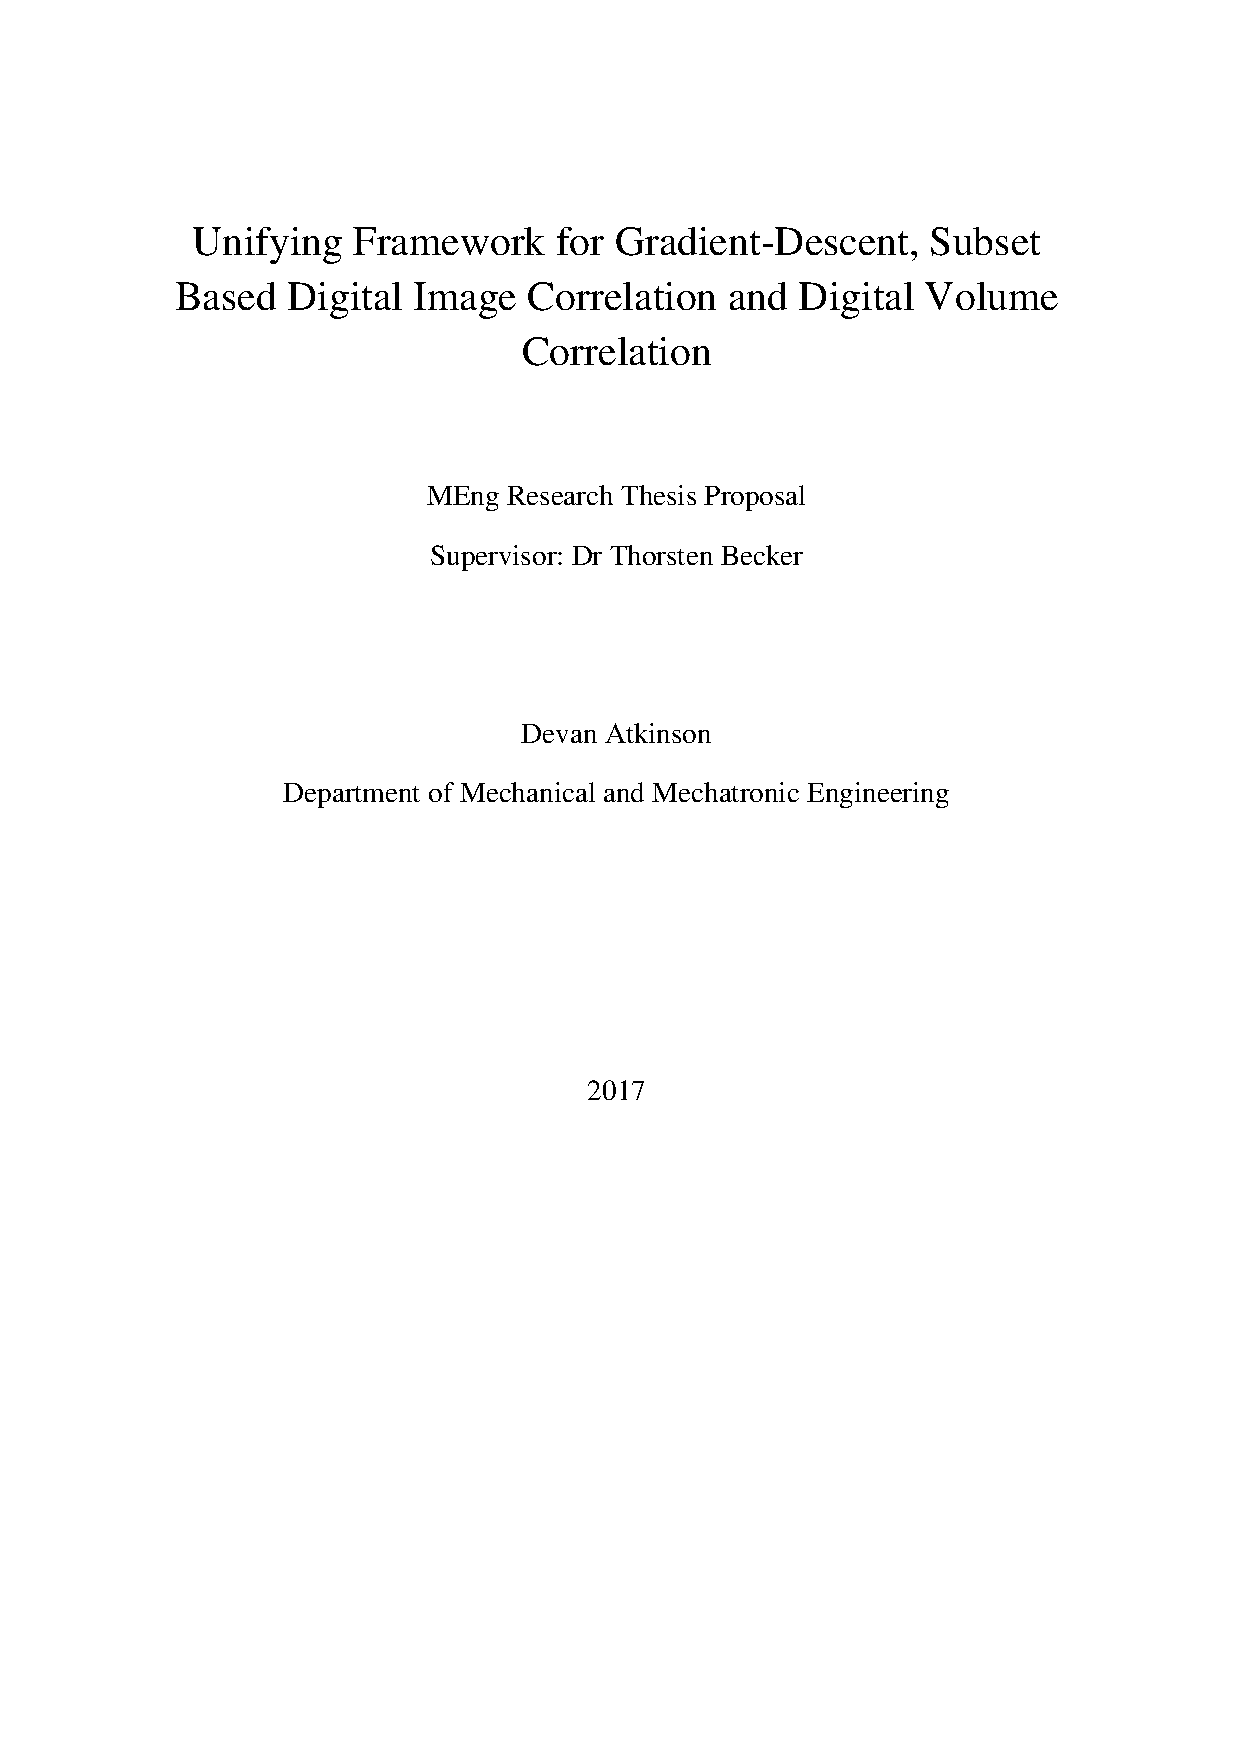
\includepdf{TitlePage.pdf}

\includepdf{plagiarism.pdf}
\chapter*{Abstract}
Digital Image Correlation (DIC) and Digital Volume Correlation (DVC) are becoming widely used tools, in the field of material science, to measure the displacements and deformations of specimens. However the high cost of commercial DIC and DVC software and the limited control offered over the correlation process in both commercial and open-source software limits its widespread adoption. This paper proposes a project which aims to create a Matlab based program capable of performing 2D DIC and DVC on a given set of images while allowing the user control over the correlation process. It is hypothesised that the different DIC algorithms use different methods to perform the same tasks in the correlation process. Thus by analysing these algorithms it is possible to combine these different methods into one program which will allow the user to select which methods to use for the various correlation tasks. If successful, this project will produce a freely available program, which offers many of the correlation methods of the different DIC algorithms, so that users will be able to perform in depth DIC and DVC analyses.

% which allows users full control over the correlation process 

% This project primarily consists of researching different DIC algorithms to determine the various methods of performing correlation and incorporating these methods into the program so that the user can choose which to use.



%  This project is motivated by the lack of freely available DIC software which allows the user to control the correlation process. This software is intended to combine most of the 2D DIC algorithms that are beneficial to material science applications into a single code. The successful completion of this project  will allow researchers of material science a comprehensive tool to determine specimen deformation from images taken of the specimen.

\tableofcontents
\listoffigures
\chapter{Introduction}


\chapter{Correlation}
The Lucas-Kanade algorithm was used in combination with the zero-mean normalised sum of squared differences correlation criteria. This correlation criteria was chosen since it takes into account offset and scaling in the light intensities of the images making the overall algorithm more robust. The Lucas-Kanade algorithm assumes that the deformation of the image is constant over a area of the image referred to as the subset. As such this algorithm tries to find the deformation field that best corrects a subset of the deformed image so that it appears to be the same as the reference image. 

\section{Correlation criteria}
Each correlation criteria is based off of a cost function which is usually a variation of the
sum of squared differences between the intensities of the reference and investigated subset.
They vary in the scaling and offset that is applied to the investigated subset’s intensity
values.


A correlation criteria is a mathematical way of quantifying how well a subset in one image matches to a subset in another image. It is used to determine whether the deformation field that has been solved for is sufficiently accurate to explain how the deformed image is related to the reference image. As such it is important that the correlation criteria reliably indicates the fit between the two subsets.

The zero-mean normalised sum of squared differences (ZNSSD) correlation criteria is one of the most robust options for a correlation criteria since it accounts for both lighting offset and scaling between the reference and deformed images. Correlation criteria are based off of a cost function which is usually a variation of the sum of squared difference between the pixel values of a subset of the reference image and a subset of the defromed image. The ZNSSD correlation criteria has the following cost function.
\begin{equation}
\label{eq:cf znssd}
  \chi_{ZNSSD}^2 = \sum_i \left( a G_i + b - F_i \right) ^2
\end{equation}
The offset $b$ and scaling $a$ can be solved for by treating it as an additional parameter of the optimisation problem. However it is preferred to determine the optimal estimates for $b$ and $a$ by taking the derivative of the cost function with respect to $a$ and $b$ separately and setting this to zero.
\begin{align}
  \frac{\partial \chi_{ZNSSD}^2 }{\partial a} &= 2 \sum_i \left( a_{opt} G_i + b- F_i \right) G_i = 0\\
  \Rightarrow a_{opt} &= \frac{\sum_i \left( F_i - b \right) G_i}{\sum_i G_i^2} \\
  \frac{\partial \chi_{ZNSSD}^2 }{\partial b} &= 2 \sum_i \left( a G_i + b_{opt} - F_i \right) = 0\\
  \Rightarrow b_{opt} &= \frac{\sum_i F_i -a G_i}{n}
\end{align}
Here $n$ is the number of pixels in the subset and $\mean{F}$ and $\mean{G}$  are the average intensity values for the reference and investigated subset respectively. These can be solved to obtain
\begin{align}
  a_{opt} &= \frac{\sum_i \mean{F_i} \mean{G_i}}{\sum_i \mean{G_i^2}}, &b_{opt}&= \mean{F} -\mean{G} \frac{\sum_i \mean{F_i} \mean{G_i}}{\sum_i \mean{G_i^2}} \\
  \text{where} \quad \quad \mean{F_i} &= F_i - \mean{F} \quad \quad \quad \quad \text{and} & \mean{G_i} &= G_i -\mean{G}
\end{align}
Substituting these into equation \ref{eq:cf znssd} results in the correlation criteria.
\begin{equation}
  \chi_{ZNSSD}^2 = \sum_i \left( \left( \frac{\sum_i \mean{F_i} \mean{G_i}}{\sum_i \mean{G_i^2}} G_i - \mean{G} \frac{\sum_i \mean{F_i} \mean{G_i}}{\sum_i \mean{G_i^2}} \right) - F_i + \mean{F} \right) ^2
\end{equation} 



\section{Warp function}
When applying DIC to to material science the deformation behaviour of materials under load must be taken into account. This is because the deformation of the material causes the speckle pattern on its surface to deform in the same way. This is an issue since the pattern contained within a subset of the reference image will be deformed in the second image which can cause difficulties in matching the two subsets.

This is solved by allowing for the subsets to deform in a similar way to that of the material by defining the allowable deformations in a warp function. The purpose of these warp functions is to transform the pixel coordinates of the reference subset so that the resulting pattern is closer to the pattern in the deformed image. For this analysis the common warp function which accounts for affine transformations is used since it is consistent with the strains that the material is expected to experience. Thus by determinig the warp function parameters for a specific subset; the strains for that subset are also determined.
\begin{equation}
  W (\bm{x},\bm{p}) = 
  \begin{bmatrix}
  x_{warp} \\
  y_{warp}
  \end{bmatrix} 
  = \begin{bmatrix}
  x + u + \frac{\partial u}{\partial x} \Delta x + \frac{\partial u}{\partial y} \Delta y \\
  y + v + \frac{\partial v}{\partial x} \Delta x + \frac{\partial v}{\partial y} \Delta y
  \end{bmatrix}.
  \label{eq:warp}
\end{equation}
Here $x$ and $y$ represent the position of the pixel in the original image, $u$ and $v$ represent the displacements in the x and y directions respectively, $\frac{\partial u}{\partial x}$ and $\frac{\partial v}{\partial y}$ represent the elongation in the x and y directions respectively, $\frac{\partial v}{\partial x}$ and $\frac{\partial u}{\partial y}$ represent the shear deformation of the subset, $\Delta x$ and $\Delta y$ are the distances from the centre of the subset to the pixel under consideration and $x_{warp}$ and $y_{warp}$ are the modified pixel coordinates after the warp has been applied.

With most subset based DIC algorithms the more complex the warp function becomes the more computationally expensive each iteration is. This is because the correlation criteria must be optimized in terms of more variables leading to more work. \todo{keep this?}

\section{Interpolation}
For DIC to be useful in the field of material science it must be able to determine displacements to sub-pixel accuracy. This requires knowing the light intensity values, within an image, between pixel locations. This is an issue because images store this information in a discrete manner. Interpolation is used to determine the light intensity values between pixels based on the light intensity values of neighbouring pixels. For the purposes of this project Matlab's built in interp2 fucntion was used to perform linear interpolation to determine the light intensity values for non-standard pixel locations where needed.




Different applications of DIC place different requirements on the DIC algorithm. Within material science applications one of the main requirements is that the displacements be tracked accurately to a very high resolution. For example to create an accurate stress-strain curve for common engineering materials a resolution on the order of $10^{-5} m/m$ is required \cite{sutton2009image}. This thus requires displacements to be determined to sub-pixel resolutions.

The issue with this is that this requires the light intensity to be continuous whereas digital images are discrete. Interpolation is used to determine the light intensities between pixels so that an approximation to the continuous form of the intensity pattern on the surface of the specimen can be calculated.

\section{Subset matching}







\chapter{Conclusion}
This document proposes a research project aimed at creating a program for Matlab that is capable of performing DIC or DVC on a given set of images. The proposed program is aimed at providing the user with full control over the correlation process so that users no longer need to treat DIC and DVC as a black box. This project is not intended to have any direct application in industry but rather to provide researchers with a comprehensive tool to perform correlation to determine material deformation.

The motivation of the project has been outlined along with literature review on DIC. The objectives of the project have also been outlined with a research plan which is aimed at achieving these objectives. A time-line for the activities of the research plan is also provided. It is evident that sufficient knowledge and resources are available for the successful completion of this project.
% \section{Outline of chapters}
\bibliography{references}
\bibliographystyle{plain}
\end{document}




% website for computer vision http://dblp.uni-trier.de/db/journals/ivc/ivc29.html


% Are you a vault dweller, cause you seem pretty S.P.E.C.I.A.L. to me





% https://drive.google.com/uc?export=download&confirm=TXgS&id=0B8ChoAcEOa4HbWxmbGFPV2M0aHM
% https://drive.google.com/uc?export=download&confirm=3xOY&id=0B8ChoAcEOa4HaEljZllabTZaeEk
% https://drive.google.com/uc?export=download&confirm=Lu4C&id=0B8ChoAcEOa4HcHZJMlZLeHdwdnc
% https://drive.google.com/uc?export=download&confirm=Qic1&id=0B2LiEl8up6X_R1V5NkF2NVhwaG8
% https://drive.google.com/uc?export=download&confirm=Qic1&id=0B2LiEl8up6X_R1V5NkF2NVhwaG8
% https://drive.google.com/uc?export=download&confirm=78XC&id=0B_q296AKMRsBUGtORW1jQ0lKQzQ


% https://drive.google.com/uc?export=download&confirm=cxmO&id=0B56v3YurenhzYTRXZGZ6MzJOWnc